Now that we have looked at the analytical solutions of our spin model, we would like to run some Monte Carlo simulations to further explore the system's properties. In the Monte Carlo simulations we will implement the Wolff Cluster Algoritm. To do this we must find the probability of a neighbouring pair of spins creating a bond; the probability of them becoming part of the same cluster. From the lectures we know that the ising model of two spins has such a "connect probability" of $p = 1 - e^{2 J \beta }$. However, in this system we have three spin states. 

To find this probability, we start out with the system's probability density in equilibrium given a set of states, see \cref{eq:W}  
\begin{equation}
    W(\sigma) = \frac{1}{Z} \exp{- \beta H(\sigma)}
    \label{eq:W}
\end{equation}

The idea behind Monte Carlo simulations is to create a stochastic process that takes us to $W(\sigma)$ as time goes to infinity. For this we can implement a transition probability, $P(\sigma \rightarrow \sigma')$, which is the probability of going from one phase to another. At the time of equilibrium one can assume a concept called \textit{detailed balance}. This states that the probability density of being in a state, $\sigma$, times the probability of going from that state to another state, $\sigma'$, equals the probability of being in $\sigma'$ times the probability of going from $\sigma'$ to $\sigma$. This is shown mathematically in \cref{eq:DB}. 
\begin{equation}
    W(\sigma)P(\sigma \rightarrow \sigma') = W(\sigma')P(\sigma' \rightarrow \sigma)
    \label{eq:DB}
\end{equation} 
It can be interpreted as the flux from one state to another is equal to the opposite flux, which seems logical considering we are in equilibrium. 

The transition probability is determined by the specific Monte Carlo algorithm implemented, and in our case it is governed by the probability of creating bonds and the probability of flipping the spin. As the probability of flipping is constant it can be ignored on both sides of the detailed balance equation. The same goes for the canonical distribution function part of $W(\sigma)$. We therefore want to create a probability density which intails the probability of creating a bond $W(\sigma, b)$. Then the detailed balance equation will become $W(\sigma, b) = W(\sigma', b)$
% Examining $Z$ gives
% \begin{align*}
%     Z &= \sum_{\{\sigma\}}\exp{-J \beta H(\sigma)}\\
%     &= \sum_{\{\sigma\}}\exp{-J \beta \sum_l \delta_{\sigma_l \sigma_{l+1}}}\\
%     &= \sum_{\{\sigma\}}\prod_l \exp{-J \beta \delta_{\sigma_l \sigma_{l+1}}}\\
%     &= \sum_{\{\sigma\}}\prod_l \exp{-J \beta} \delta_{\sigma_l \sigma_{l+1}} + (1-\delta_{\sigma_l \sigma_{l+1}})\\
%     &= \sum_{\{\sigma\}}\sum_{\{b\}} \prod_l \exp{-J \beta} \delta_{\sigma_l \sigma_{l+1}} \bclosed{p \delta_{b_l,1} + (1-p)\delta_{b_l,0}} + (1-\delta_{\sigma_l \sigma_{l+1}})\delta_{b_l,0}\\
% \end{align*}
Ignoring $Z$ gives
\begin{align*}
    W(\sigma) &= \exp{-J \beta H(\sigma)}\\
    &= \exp{-J \beta \sum_l \delta_{\sigma_l \sigma_{l+1}}}\\
    &= \prod_l \exp{-J \beta \delta_{\sigma_l \sigma_{l+1}}}\\
    &= \prod_l \exp{-J \beta} \delta_{\sigma_l \sigma_{l+1}} + (1-\delta_{\sigma_l \sigma_{l+1}})\\
    &= \sum_{\{b\}} \prod_l \exp{-J \beta} \delta_{\sigma_l \sigma_{l+1}} \bclosed{p \delta_{b_l,1} + (1-p)\delta_{b_l,0}} + (1-\delta_{\sigma_l \sigma_{l+1}})\delta_{b_l,0}\\
    &= W(\sigma, b)
\end{align*}
We have now implemented the probability for creating a bond, $p$ (not to be confused with the probability density $P(\sigma \rightarrow \sigma')$). 

Now considering a two-particle system, we analyse the various values of $W(\sigma, b)$, see~\cref{tab:W}.

\begin{table}[]
    \def\arraystretch{1.25}
    \centering
    \begin{tabular}{|ccc|}
        \hline
        \multicolumn{3}{|c|}{$W(\sigma, b)$}                                                                                                      \\ \hline
        \multicolumn{1}{|c|}{$p \exp{J \beta}$} & \multicolumn{1}{c|}{$(1-p) \exp{J \beta}$} & 1   \\ \hline
        \multicolumn{1}{|c|}{0-0}                                             & \multicolumn{1}{c|}{0 0}                                                 & 0 1 \\ \hline
        \multicolumn{1}{|c|}{1-1}                                             & \multicolumn{1}{c|}{1 1}                                                 & 0 2 \\ \hline
        \multicolumn{1}{|c|}{2-2}                                             & \multicolumn{1}{c|}{2 2}                                                 & 1 0 \\ \hline
        \multicolumn{1}{|c|}{}                                                & \multicolumn{1}{c|}{}                                                    & 1 2 \\ \hline
        \multicolumn{1}{|c|}{}                                                & \multicolumn{1}{c|}{}                                                    & 2 0 \\ \hline
        \multicolumn{1}{|c|}{}                                                & \multicolumn{1}{c|}{}                                                    & 2 1 \\ \hline
    \end{tabular}
    \caption{Table of possible $W(\sigma,b)$ values in a two partcile system. The "-" refers to a bond between the spins.}
    \label{tab:W}
\end{table}

From detailed balance we can now set $W(\sigma, b)$ from the instance where the spins are equal to eachother equal to the $W(\sigma, b)$ where they are different and solve for $p$
\begin{align*}
    W(\sigma, b) &= W(\sigma', b)\\
    (1-p) \exp{J \beta} &= 1\\
    p &= 1 - \exp{-J \beta} 
\end{align*}

Comparing with the connnect probability of the two spin ising model, this probability is smaller given the same $T$ (for $T>0$). This seems intuitive considering we are now working with three spins, as opposed to two, and there is a smaller chance two spins are equal, which is necessary for a bond to be created.\\ 
Now, with the connect probability calculated the implementation of the Monte Carlo simulations can find place. 


\section*{b)}
    After conducting the Monte Carlo simulations we want to compare the results from the simulations and the analytical solutions performed in the previous part. To do this, we examine the correlation function $C(r)$. To numerically calculate the correlation function (and later on other expressions including ensemble averages), we assume ergodicity of the system, ant take the ensamble averages over "time". See~\cref{fig:C} for the plot of $C(r)$. 
    \begin{figure}[h]
        \centering
        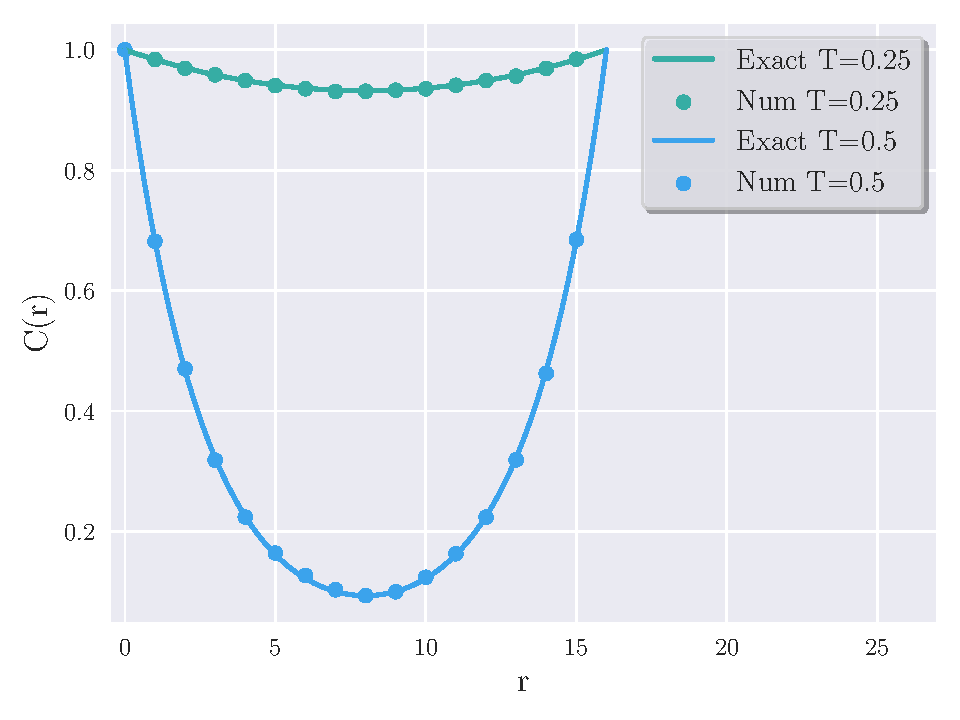
\includegraphics[width=.49\textwidth]{../figs/plot_b.pdf}
        \caption{Comparing analytical and numerical solution of $C(r)$ of a 1D lattice system with 16 spins.}
        \label{fig:C}
    \end{figure}
   
    As can be seen in the plot, the results coincide. We can again see that the correlation function goes to 1 as $r$ goes to 0 and as it goes to the end of the lattice (analytically this was as $r \rightarrow \infty$). Considering our system has periodic boundry conditions, this seems logical. For a higher temperature (T=0.5 in the plot) the correlation varies more. As the temperature increases, the system tends to be more disordered and less correlation is therefore expected. In the numerical case, the temperature is included in the possibility of creating bond between spins, $p = 1 - \exp{-1/T}$. When T is increased, the probability of creating bonds decreases which then leads to a bigger spread in states.  


\section*{c)}
    From this point on we will consider a system of a $L$x$L$ 2D lattice with periodic bondries conditions in both directions. 
    
    To test our results from the analytical part where we concluded that $\expval{m}=0$ for all temperatures we will plot \expval{m} as a function of T. We implement a system of $L=16$ in our simulations. See~\cref{fig:m_T} 

    \begin{figure}[h!]
        \centering
        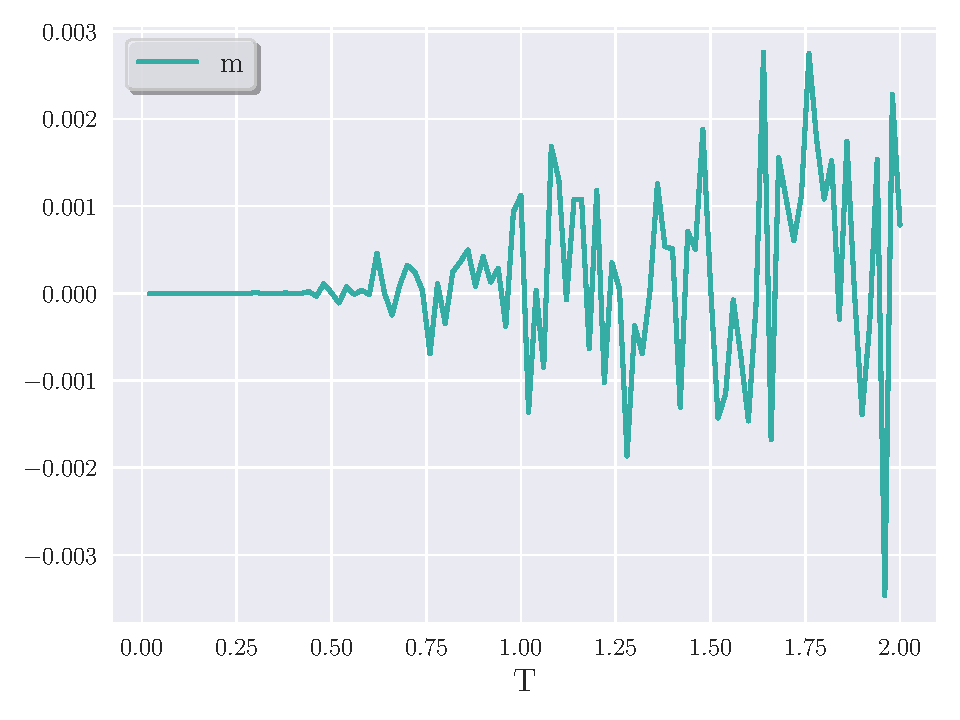
\includegraphics[width=0.44\textwidth]{../figs/m_T_2.pdf}\\
        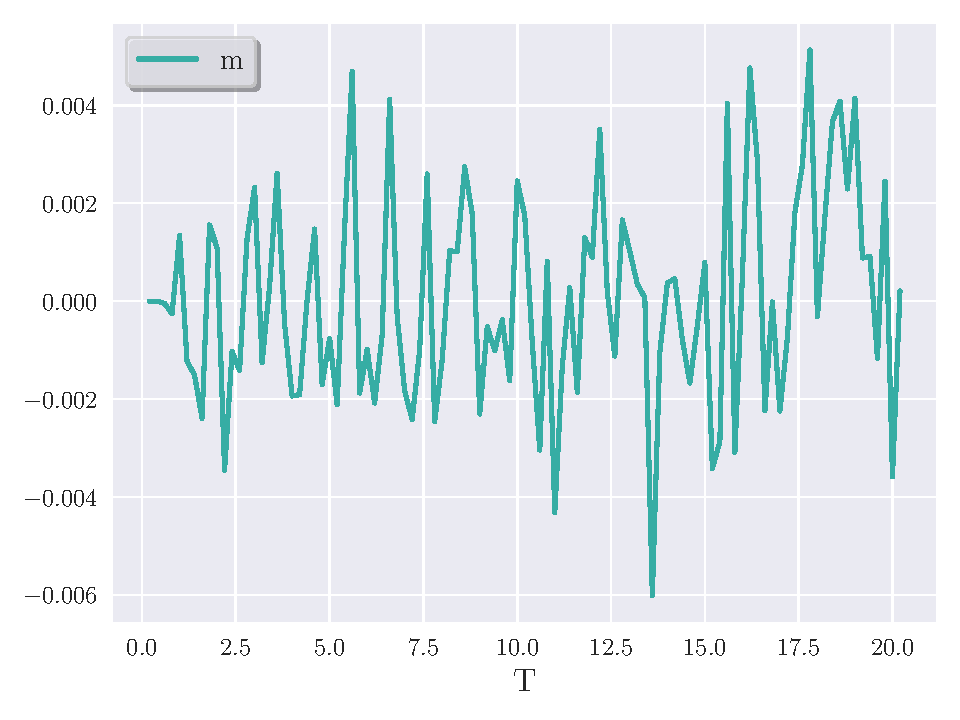
\includegraphics[width=0.44\textwidth]{../figs/m_T_20.pdf}
        \caption{Plots of \expval{m} as a function of temperature.}
        \label{fig:m_T}
    \end{figure}

    In the plots it is shown that \expval{m} oscillates around 0 for all Ts. However, it oscillates considerably more for higher temperatures; there is a shift around T=0.5. This can be explained by the numerical approach. Calculating \expval{m} numerically means summing over a finite number of $m_j$-values. Even though these values are supposed to sum to zero, analytically, this is not necessarily the case in a system of 16x16 spins. The increase in oscilations as T increases can again be explained by the increase in disorder.   



\section*{d)}
    In addition to looking at the average magnetisation per site, \expval{m}, it could be interesting to look at the average magnetisation squared per site, \expval{|m|^2}. In that case it might not sum to 0, and we can further inspect its properties. See~\cref{fig:m2_T} for the results. 
    % \begin{figure}
    %     \centering
    %     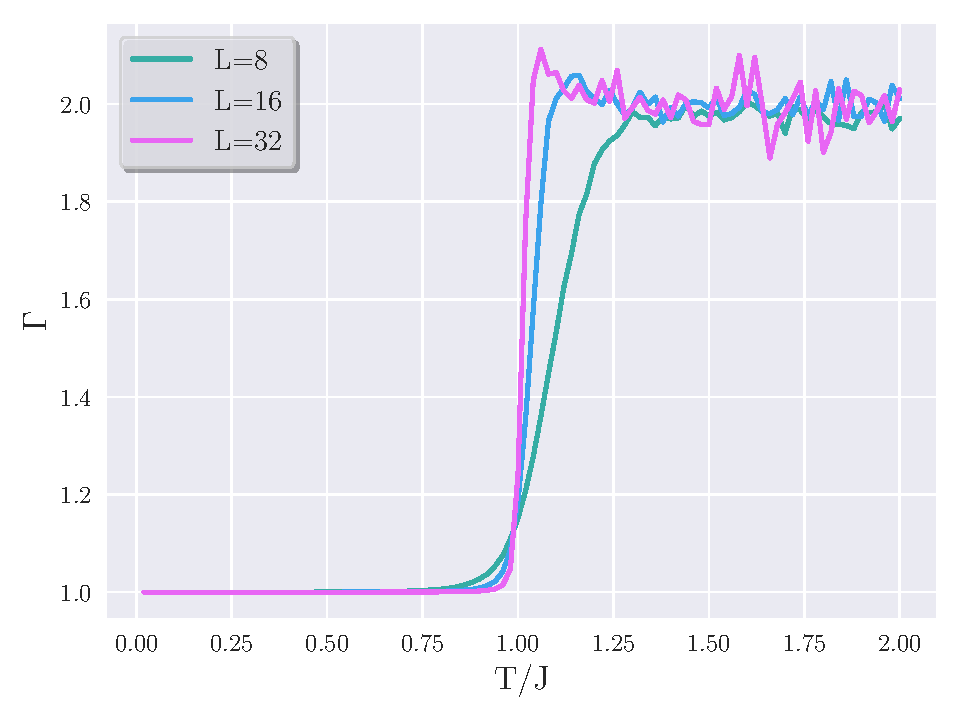
\includegraphics[width=0.44\textwidth]{../figs/gamma_T.pdf}
    %     \caption{Plots of \expval{|m|^2} as a function of temperature.}
    %     \label{fig:m2_T}
    % \end{figure}
    \begin{figure*}
        \centering
        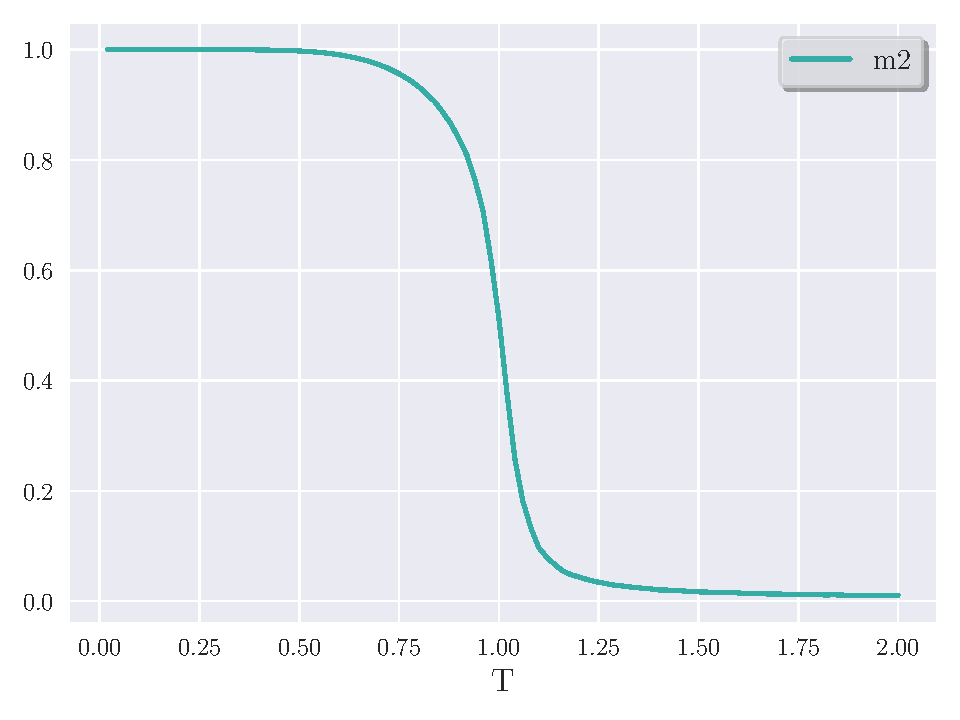
\includegraphics[width=0.44\textwidth]{../figs/m2_T_2.pdf}
        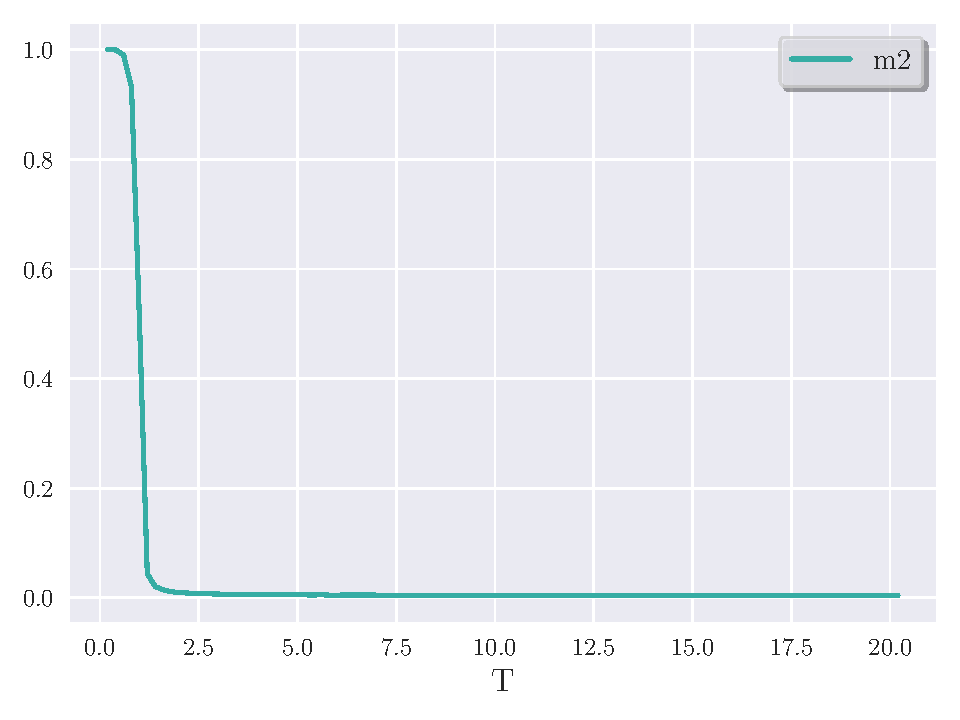
\includegraphics[width=0.44\textwidth]{../figs/m2_T_20.pdf}
        \caption{Plots of \expval{|m|^2} as a function of temperature.}
        \label{fig:m2_T}
    \end{figure*}
    For low T \expval{|m|^2} is equal to 1, then around T=1 it continuously goes to 0. This means that for low T, the magnetisation per site sums to 0 only when taking the ensemble average, and that for high T the magnetisation per site is equal to 0 by itself. 
    
    This can be interpreted as the system having some magnetic property at low T. This coincides with the theory of low Ts yielding an ordered state. Hoewever, taking the ensamble average of these possible low T states of the system makes the magnetisation per site sum to zero. In other words, there is no favourability of one of the spin states, 0, 1, or 2 across the ensembles. On the other hand, for high Ts, the squared magnetisation per site is 0, meaning the system has no magnetic properties (in accordance with high T yielding unordered states). There seems to be a phase transition around T=1; going from the ordered to the unordered state. 


\section*{e)}
    As we want to further inspect the critical temperature of a phase transition in this system, we will introduce the dimensionless quantity $\Gamma$, which is a ratio of moments of the magnetisation
    \begin{equation}
        \Gamma = \frac{\expval{|m|^4}}{\expval{|m|^2}^2}
        \label{eq:gamma}
    \end{equation}
    Evaluating $\Gamma$ as a function of $T/J$ for various values of $L$ can tell us at which temperatures the system is scale free. Eg. if two graphs, of two different $L$-values, cross, then the $T$-value at which they cross results in a system where $\Gamma$ is independt of the scale of the system. From the theory, we know that this is a property of a critical temperature. Mathemmatically this can be shown as 
    \begin{align*}
        \Gamma (t, L^{-1}) = s^d \Gamma (ts^{yt}, sL^{-1})
    \end{align*}
    where $t = \frac{T - T_c}{T_c}$.\\
    Setting $s=L$ gives 
    \begin{align*}
        \Gamma (t, L^{-1}) = L^d \Gamma (tL^{yt}, 1)
    \end{align*}
    which results in the right hand side being a function of only one variable. We rename this function to
    \begin{align*}
        g(x) = g(tL^{yt}) = \Gamma (tL^{yt}, 1)
    \end{align*} 
    and taylor expand around 0 (which incidentially is the critical point). This gives us
    \begin{align*}
        \frac{\Gamma (t, L^{-1})}{L^d} = g(0) + tL^{yt}g'(0)
    \end{align*}
    Setting $t=0$ then gives 
    \begin{align*}
        \frac{\Gamma (t, L^{-1})}{L^d} = g(0)
    \end{align*}
    Which shows that at the critical temperature the $\Gamma$-function is independent of the system size, $L$. 


\section*{f)}
    Testing the theory above we now plot $\Gamma$ as a function of $T$ for various $L$, see~\cref{fig:gamma_T}. 
    \begin{figure*}
        \centering
        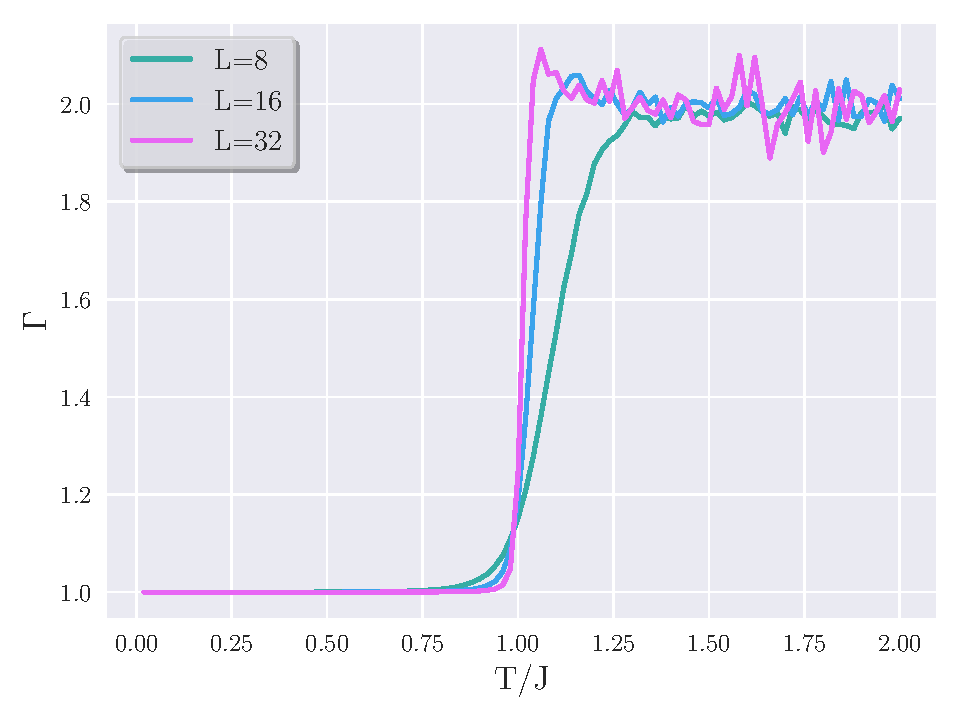
\includegraphics[width=0.44\textwidth]{../figs/gamma_T.pdf}
        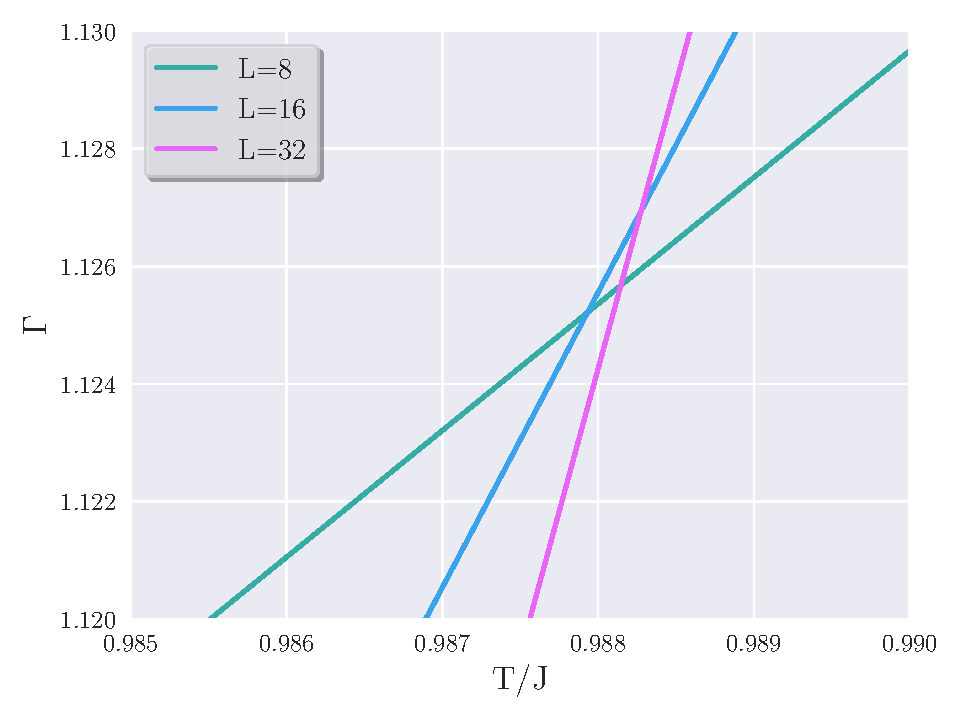
\includegraphics[width=0.44\textwidth]{../figs/gamma_T_zoom.pdf}
        \caption{Plots of $\Gamma$ as a function of temperature.}x
        \label{fig:gamma_T}
    \end{figure*}
    The exact results of the critical temperature is $T_c/J = \frac{1}{ln(1+\sqrt{3})} \approx 0.9950$. As can be seen in the plots, the intersection-values coincide very well with the exact results. However, in theory there should only be one intersection, and in the plots two intersections can be seen (ignoring the intersections after the phase change which is due to numerical oscilations as previously discussed). One could assume that this is because of the finiteness of the system which we are working with; that the bigger the system, the closer we are to the "real" critical temperature. However, this is not necessarily the case as there could be some hidden parameters which we have not taken into consideration.  